% Generated by tools/paper/render.py from main_text.py; edit the source there, not this file.
\begin{figure*}[t]
\centering
\resizebox{\textwidth}{!}{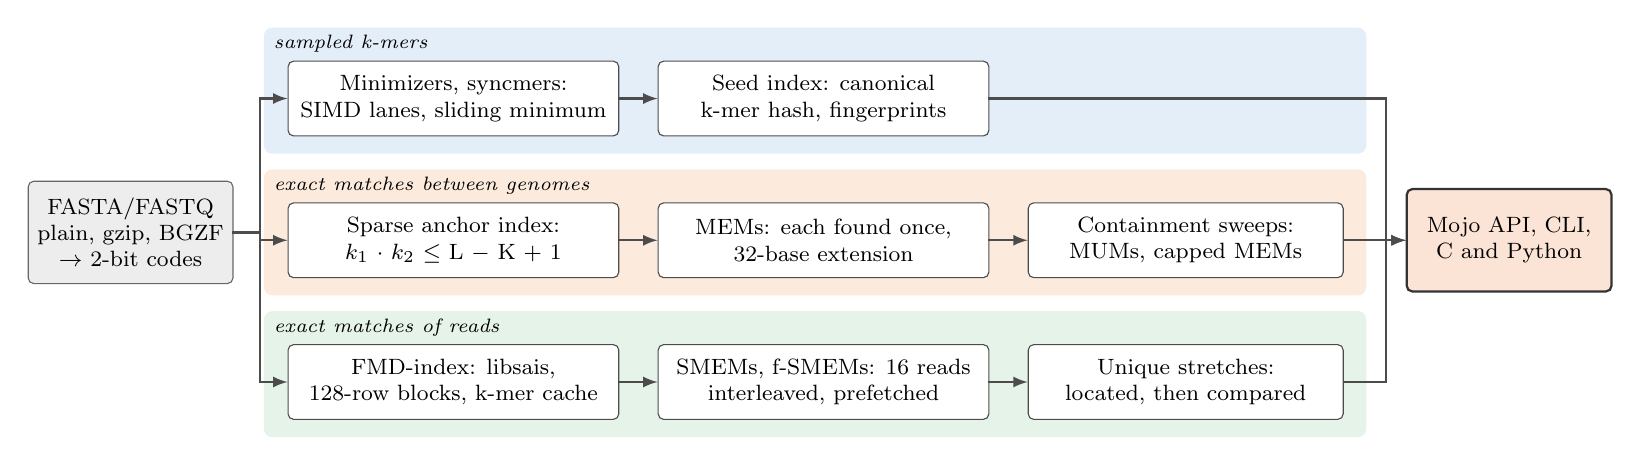
\begin{tikzpicture}
\fill[fill={rgb,255:red,227;green,238;blue,249}, rounded corners=3pt] (3.0,3.55) rectangle (17.0,5.15);\node[anchor=north west, font=\scriptsize\itshape, inner sep=2pt] at (3.05,5.130000000000001) {sampled k-mers};
\fill[fill={rgb,255:red,252;green,235;blue,221}, rounded corners=3pt] (3.0,1.75) rectangle (17.0,3.35);\node[anchor=north west, font=\scriptsize\itshape, inner sep=2pt] at (3.05,3.33) {exact matches between genomes};
\fill[fill={rgb,255:red,229;green,243;blue,232}, rounded corners=3pt] (3.0,-0.05) rectangle (17.0,1.55);\node[anchor=north west, font=\scriptsize\itshape, inner sep=2pt] at (3.05,1.53) {exact matches of reads};
\node[draw=black!60, fill={rgb,255:red,237;green,237;blue,237}, rounded corners=2pt, align=center, font=\footnotesize, inner sep=2pt, minimum width=2.6cm, minimum height=1.3cm, anchor=west] (input) at (0.0,2.55) {FASTA/FASTQ\\plain, gzip, BGZF\\$\to$ 2-bit codes};
\node[draw=black!70, fill={rgb,255:red,255;green,255;blue,255}, rounded corners=2pt, align=center, font=\footnotesize, inner sep=2pt, minimum width=4.2cm, minimum height=0.95cm, anchor=west] (window) at (3.3,4.25) {Minimizers, syncmers:\\SIMD lanes, sliding minimum};
\node[draw=black!70, fill={rgb,255:red,255;green,255;blue,255}, rounded corners=2pt, align=center, font=\footnotesize, inner sep=2pt, minimum width=4.2cm, minimum height=0.95cm, anchor=west] (seedindex) at (8.0,4.25) {Seed index: canonical\\k-mer hash, fingerprints};
\node[draw=black!70, fill={rgb,255:red,255;green,255;blue,255}, rounded corners=2pt, align=center, font=\footnotesize, inner sep=2pt, minimum width=4.2cm, minimum height=0.95cm, anchor=west] (anchors) at (3.3,2.45) {Sparse anchor index:\\$k_1$ $\cdot$ $k_2$ $\le$ L $-$ K + 1};
\node[draw=black!70, fill={rgb,255:red,255;green,255;blue,255}, rounded corners=2pt, align=center, font=\footnotesize, inner sep=2pt, minimum width=4.2cm, minimum height=0.95cm, anchor=west] (extend) at (8.0,2.45) {MEMs: each found once,\\32-base extension};
\node[draw=black!70, fill={rgb,255:red,255;green,255;blue,255}, rounded corners=2pt, align=center, font=\footnotesize, inner sep=2pt, minimum width=4.0cm, minimum height=0.95cm, anchor=west] (sweeps) at (12.7,2.45) {Containment sweeps:\\MUMs, capped MEMs};
\node[draw=black!70, fill={rgb,255:red,255;green,255;blue,255}, rounded corners=2pt, align=center, font=\footnotesize, inner sep=2pt, minimum width=4.2cm, minimum height=0.95cm, anchor=west] (fmd) at (3.3,0.65) {FMD-index: libsais,\\128-row blocks, k-mer cache};
\node[draw=black!70, fill={rgb,255:red,255;green,255;blue,255}, rounded corners=2pt, align=center, font=\footnotesize, inner sep=2pt, minimum width=4.2cm, minimum height=0.95cm, anchor=west] (search) at (8.0,0.65) {SMEMs, f-SMEMs: 16 reads\\interleaved, prefetched};
\node[draw=black!70, fill={rgb,255:red,255;green,255;blue,255}, rounded corners=2pt, align=center, font=\footnotesize, inner sep=2pt, minimum width=4.0cm, minimum height=0.95cm, anchor=west] (unique) at (12.7,0.65) {Unique stretches:\\located, then compared};
\node[draw=black!80, thick, fill={rgb,255:red,251;green,227;blue,214}, rounded corners=2pt, align=center, font=\footnotesize, inner sep=2pt, minimum width=2.6cm, minimum height=1.3cm, anchor=west] (api) at (17.5,2.45) {Mojo API, CLI,\\C and Python};
\draw[-latex, thick, black!70] (2.60,2.55) -- (2.95,2.55) -- (2.95,4.25) -- (3.30,4.25);
\draw[-latex, thick, black!70] (2.60,2.55) -- (2.95,2.55) -- (2.95,2.45) -- (3.30,2.45);
\draw[-latex, thick, black!70] (2.60,2.55) -- (2.95,2.55) -- (2.95,0.65) -- (3.30,0.65);
\draw[-latex, thick, black!70] (7.50,4.25) -- (8.00,4.25);
\draw[-latex, thick, black!70] (7.50,2.45) -- (8.00,2.45);
\draw[-latex, thick, black!70] (12.20,2.45) -- (12.70,2.45);
\draw[-latex, thick, black!70] (7.50,0.65) -- (8.00,0.65);
\draw[-latex, thick, black!70] (12.20,0.65) -- (12.70,0.65);
\draw[-latex, thick, black!70] (12.20,4.25) -- (17.25,4.25) -- (17.25,2.45) -- (17.50,2.45);
\draw[-latex, thick, black!70] (16.70,2.45) -- (17.50,2.45);
\draw[-latex, thick, black!70] (16.70,0.65) -- (17.25,0.65) -- (17.25,2.45) -- (17.50,2.45);
\end{tikzpicture}}
\caption{The sporos library. Input is parsed and coded once; three engines compute sampled k-mers and the seed index that looks them up (top), MEMs, MUMs and frequency-capped MEMs between genomes (middle), and SMEMs and f-SMEMs of reads (bottom), behind Mojo, command-line, C and Python interfaces.}\label{fig:overview}
\end{figure*}
